\documentclass[../ManualeSviluppatore.tex]{subfiles}

\begin{document}
\section{Per iniziare}

	Nel caso in cui si voglia utilizzare o estendere il codice di CLIPS si consiglia di seguire i passi di seguito descritti.

	\subsection{IDE}
		È consigliato aprire ed eventualmente modificare il progetto con l'IDE Android Studio, ossia l'IDE utilizzato ufficialmente nello sviluppo. La versione con cui è stato sviluppato il progetto è la 1.5.1. Questa sezione farà riferimento a tale versione.
		
		Android Studio è disponibile gratuitamente al seguente link:
		\begin{quote}
			\centering
			\url{http://developer.android.com/sdk/index.html}
		\end{quote}
		
		\paragraph*{Nota:} 
			Il progetto non è stato provato su Android Studio con versioni successive o precedenti, non dovrebbe portare elevate differenze per le versioni successive.
		
		
		
		
	\subsection{Download del progetto}
		\paragraph*{}
			Per poter accedere al codice è necessario accedere al link:
		\begin{quote}
			\centering
			\url{https://github.com/LeafSWE/clips}
		\end{quote}

		\paragraph*{}
			Successivamente cliccare \textbf{DOWNLOAD ZIP} e \textbf{SALVA}:
			
			\begin{figure} [h]
				\centering
				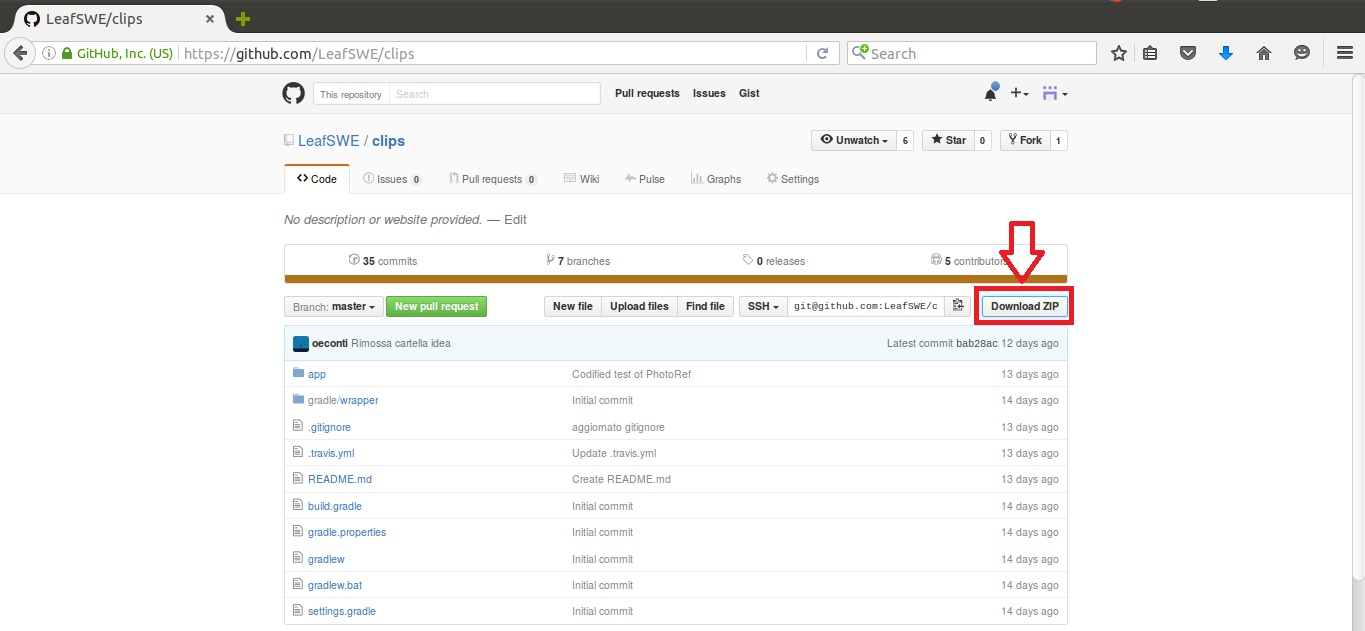
\includegraphics[scale=0.34]{img/DownloadZip}
				\label{fig:DownloadZip}
				\caption{Download progetto da Github}
			\end{figure}
			
			\begin{figure} [h]
				\centering
				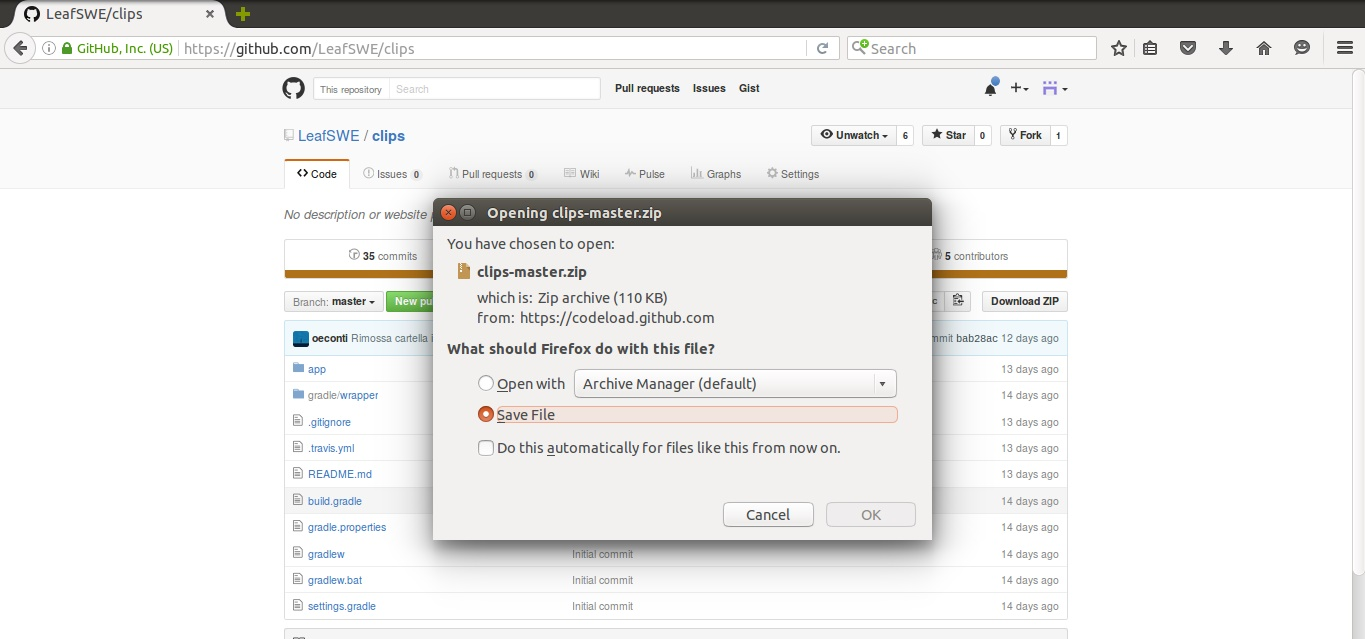
\includegraphics[width=\textwidth]{img/Download}
				\label{fig:DownloadZip2}
				\caption{Download file progetto da Github}
			\end{figure}
			
		\paragraph*{}
			Scaricato il file \verb|clips-master.zip| estrarlo con il tool per l'estrazione file preferito:
			
			\begin{figure} [h]
				\centering
				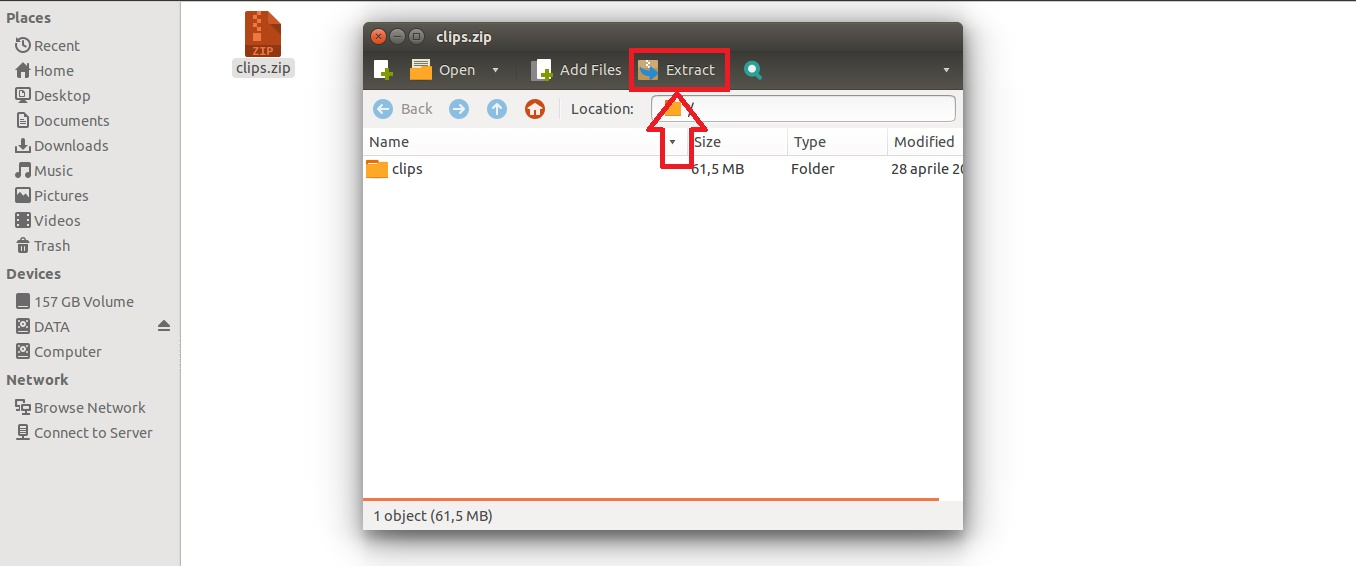
\includegraphics[width=\textwidth]{img/EstraiZip}
				\label{fig:EstraiZip}
				\caption{Estrazione file zip}
			\end{figure}
			
			
		
	\newpage	
	\subsection{Aprire il progetto con Android Studio}
		Aprire Android Studio e selezionare \textbf{Opening an existing Android Studio project}:
		
		\begin{figure} [h]
			\centering
			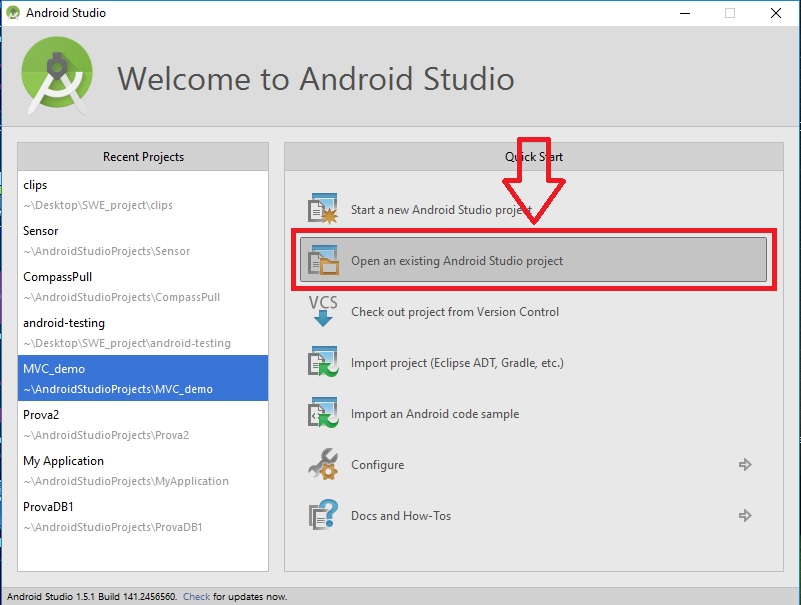
\includegraphics[scale=0.4]{img/AprireProgetto}
			\label{fig:AprireProgetto}
			\caption{Aprire il progetto con Android Studio}
		\end{figure}
		
		\paragraph*{}
			Selezionare, seguendo il giusto path, la cartella del progetto \verb|clips-master|. Attendere la \textbf{Build project info} di Gradle. Anche quando Android Studio è aperto attendere la conclusione del processo di Gradle:
			
		\begin{figure} [h]
			\centering
			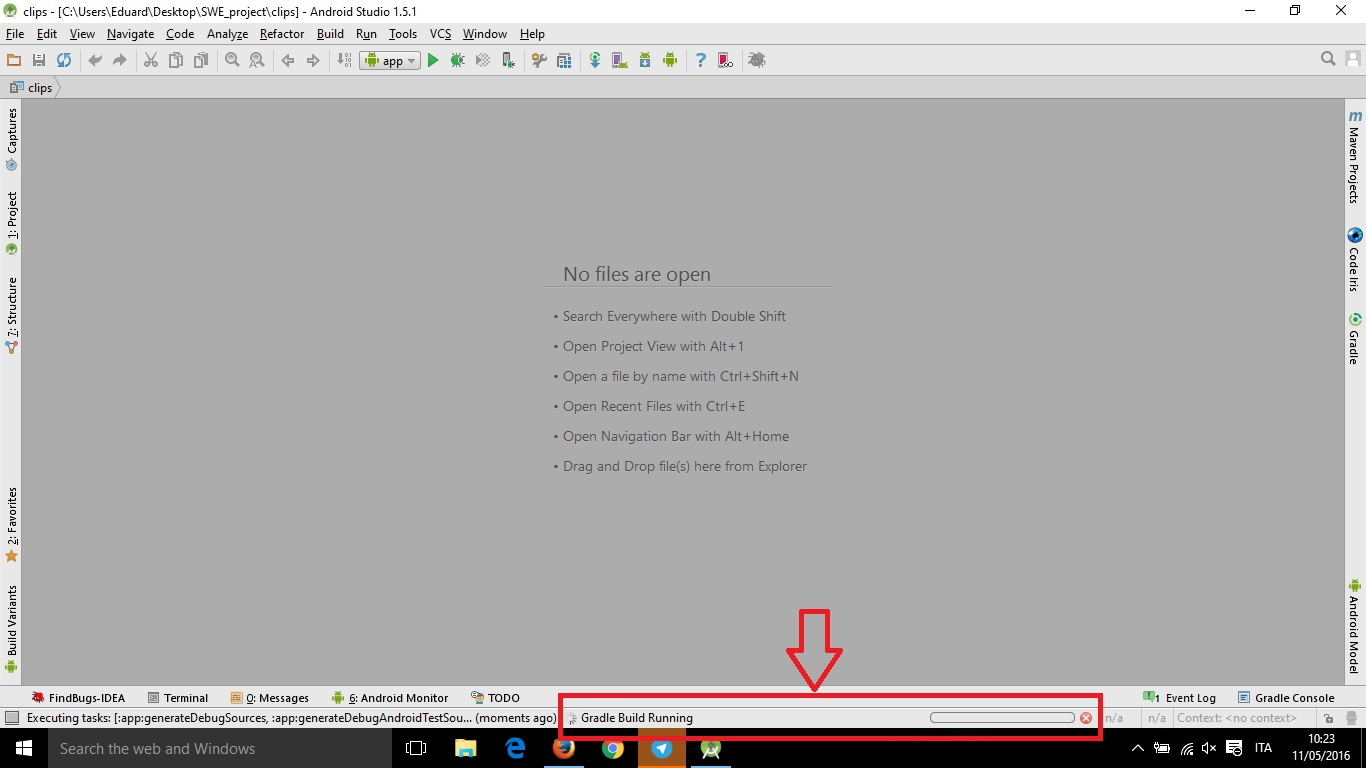
\includegraphics[scale=0.34]{img/BuildGradle}
			\caption{Build project info di Gradle}
			\label{fig:BuildGradle}
		\end{figure}
		
		\paragraph*{Nota:}
			Nel caso in cui il processo di Gradle fallisca seguire le indicazioni nella sezione \ref{subsec:Gradle}:
			
		\begin{figure} [h]
			\centering
			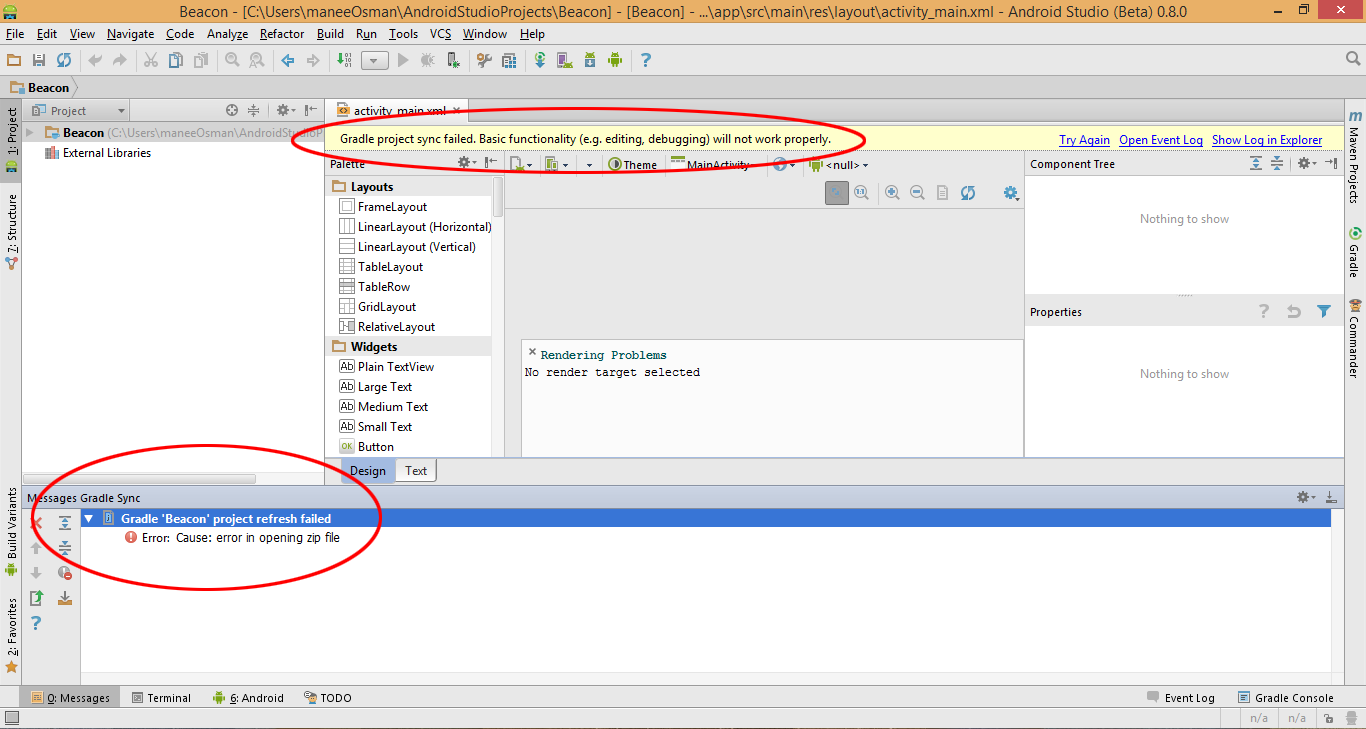
\includegraphics[width=\textwidth]{img/GradleError}
			\label{fig:GradleError}
			\caption{Errore build project info di Gradle}
		\end{figure}
		

\end{document}